\documentclass{article}
\usepackage[utf8]{inputenc}    % For UTF-8 character encoding
\usepackage[T1]{fontenc}       % For proper font encoding
\usepackage{lmodern}           % Improved font rendering
\usepackage{amsmath}   % For advanced mathematical formatting
\usepackage{amssymb}   % For mathematical symbols
\usepackage{geometry}  % Adjust page margins
\usepackage{enumerate} % For custom lists
\usepackage{xcolor}  % for coloring
\usepackage{amsthm}
\usepackage{pdfpages}
\newtheorem{theorem}{Theorem}[section]
\newtheorem{lemma}[theorem]{Lemma}
\newtheorem{corollary}[theorem]{Corollary}
\newtheorem{definition}[theorem]{Definition}
\usepackage{listings}  % for code listings

\lstset{frame=tb,
  language=C,
  aboveskip=3mm,
  belowskip=3mm,
  showstringspaces=false,   
  columns=flexible,
  basicstyle={\small\ttfamily},
  numbers=none,
  numberstyle=\tiny\color{gray},
  keywordstyle=\color{blue},
  commentstyle=\color{brown},
  stringstyle=\color{orange},
  breaklines=true,
  breakatwhitespace=true,
  tabsize=3
}
\geometry{top=1in, bottom=1in, left=1in, right=1in}

\begin{document}

\title{}
\author{Wang Xiyu}
\date{}
\maketitle
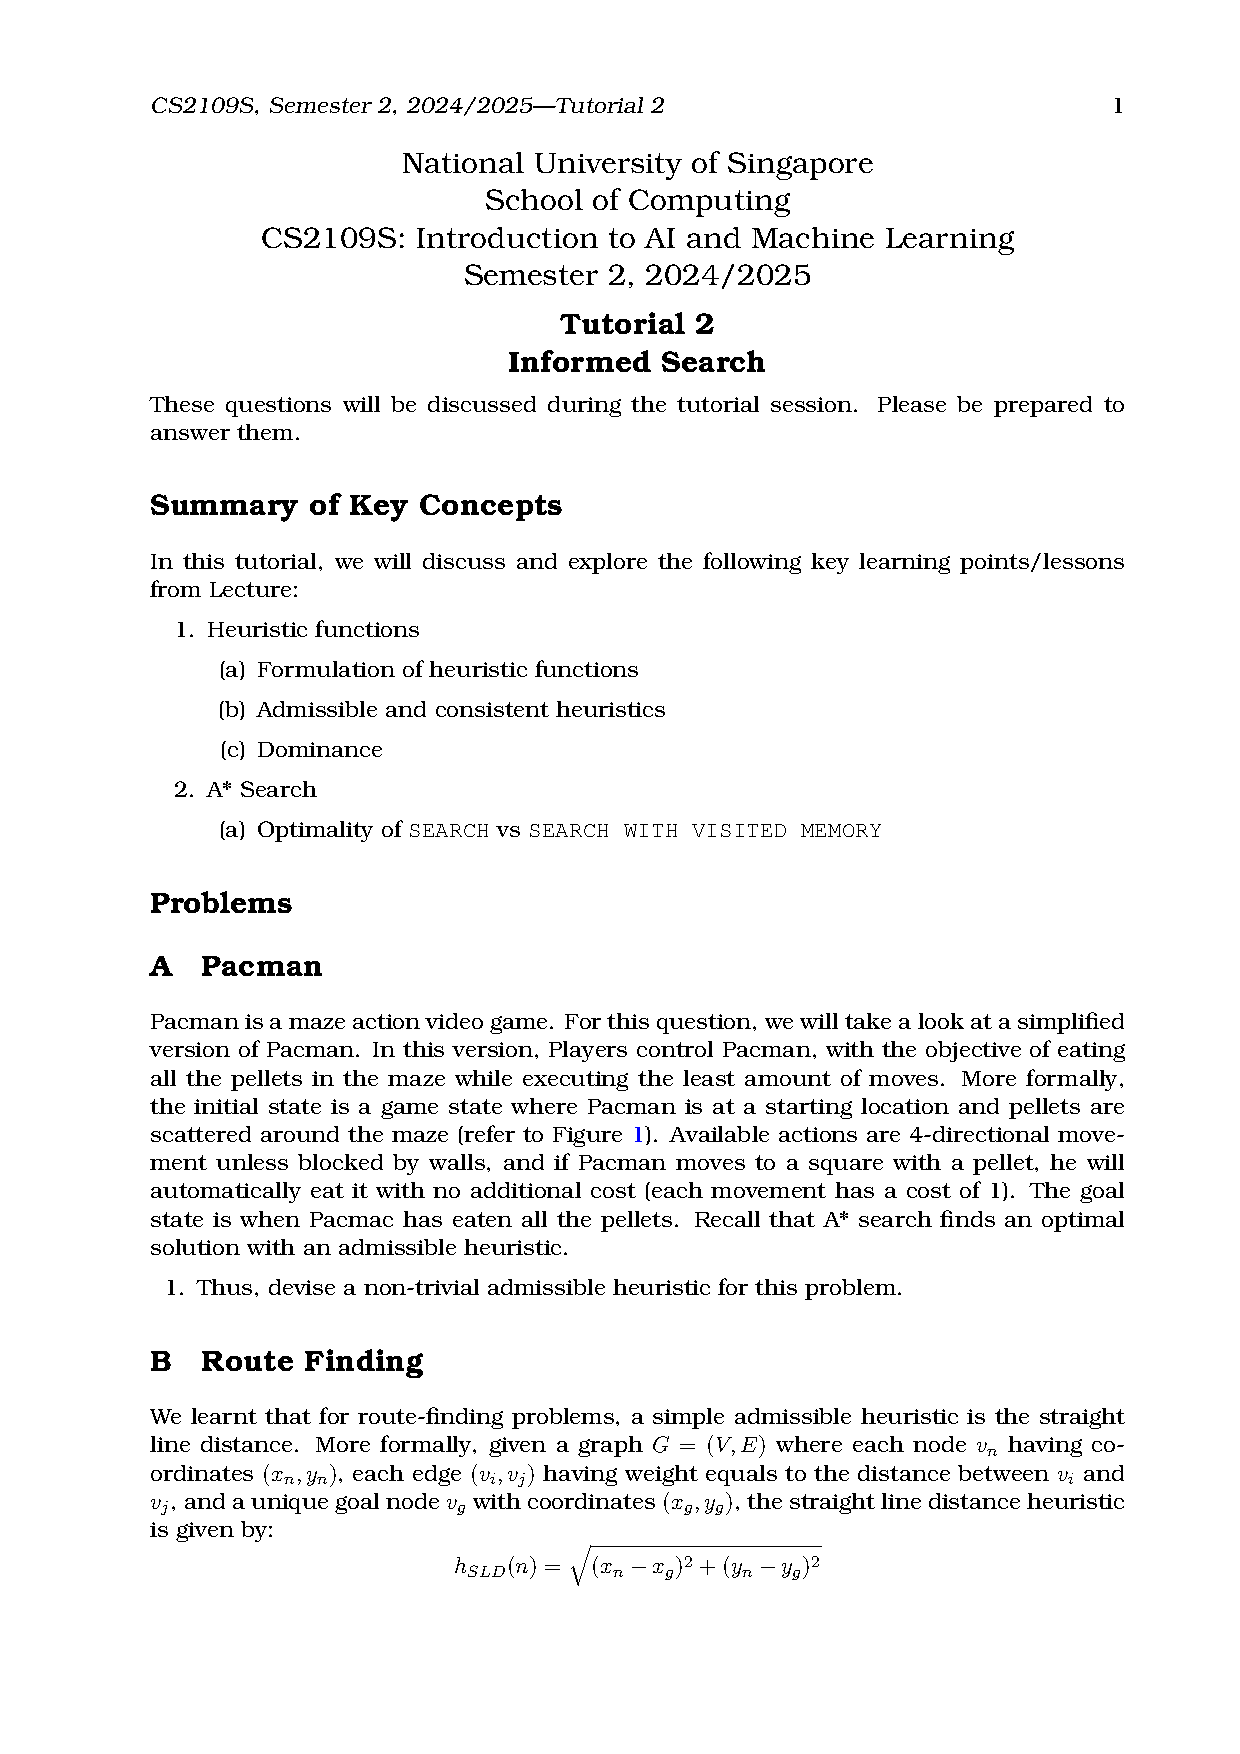
\includepdf[pages=1]{Tutorial2.pdf}
\section{A} 
\begin{itemize}
    \item State representation: current board, including remaning pellets and the position of the Pacman
    \item Action: horizontal or vertical move 
    \item Representation invariant: 
\end{itemize}
A non-trivial heuristic that is admissible: 
\begin{equation}
    h(n) = \text{no. of pellects remaining}
\end{equation}
Justification: Apparently $h(0) = 0$, and one move can consume at most one pellets, thus $\forall n \in State, h(n) \leq h^*(n)$.
\begin{equation}
    h(n) = 
\end{equation}
\includepdf[pages=2]{Tutorial2.pdf}
\section{B}
\subsection{}
\begin{proof}
    WLOG, suppose $|x_n - x_g| \geq |y_n - y_g|$. $\forall y_n, y_g \in \mathbb{R}, |y_n - y_g| \geq 0$.\newline 
    $\forall x_n, x_g, y_n, y_g \in \mathbb{R}$: 
    \[\sqrt{(x_n - x_g)^2 + (y_n - y_g)^2} \geq \sqrt{(x_n - x_g)^2} \geq |x_u - x_g|\]
    Given $h(n) = \sqrt{(x_n - x_g)^2 + (y_n - y_g)^2}$ is admissible, 
    $h(n) = max(|x_n - x_g|, |y_n - y_g|)$ is also admissible.\newline

    Suppose $\exists k \in State$, $h(n) = max(|x_n - x_g|, |y_n - y_g|)$, 
    $h(k) = max(|x_k - x_g|, |y_k - y_g|)$, if $max(|x_k - x_g|, |y_k - y_g|) \geq max(|x_n - x_g|, |y_n - y_g|)$, trivial.
    Otherwise, given $h(n) = \sqrt{(x_n - x_g)^2 + (y_n - y_g)^2}$ is admissible, 
    \[c(n, k) \geq \sqrt{(x_n - x_k)^2 + (y_n - y_k)^2}\] 
    \[c(n, k) + h(k) \geq \sqrt{(x_n - x_k)^2 + (y_n - y_k)^2} + max(|x_k - x_g|, |y_k - y_g|)\]
    \[c(n, k) + h(k) \geq max(|x_n - x_k|, |y_n - y_k|) + max(|x_k - x_g|, |y_k - y_g|) \geq max(|x_n - x_g|, |y_n - y_g|) \]
    Thus $h_1(n)$ is consistent.

\end{proof}
\subsection{}
Counter example: When diagnoal moves are allowed.

\subsection{} 
% $h_1(n)$. Consistent and Admissible, also lower computation cost than $h(n)$
\textcolor{red}{$h(n)$ as it dominants $h_1(n)$. Prioritize choosing the dominant heuristic.}
\section{C}
Prove: Consistency implies admissibility\newline
Admissibility
\begin{equation}
    \forall n \in State, h(n) \leq \sum_{i = start}^{goal}c(i', a, i)
\end{equation}
Consistency
\begin{equation}
    \forall n \in State, \forall a \in Action, h(n) \leq h(n') + c(n', a, n)
\end{equation}
\begin{proof}
    Base case: $n_{start} \vdash n_{goal}$, $h(n_{goal}) = h^*(n_{goal})$, 
    \[h(n_{start}) \leq c(n_{start}, n_{goal}) + h^*(n_{goal}) = h^*(n_{start})\]
    Inductive case: suppose n is of k distance away from $n_{goal}$ on the optimal path from $n_{start}$. From the base case we have, 
    \[h(n_k) \leq h^*(n_k)\]
    \[h(n_{k-1}) \leq h(n_k) + c(n_{k-1}, n_k) \leq h^*(n_k) + c(n_{k-1}, n_k) = h^*(n_{k-1})\]


\end{proof}
\section{D}
\subsection{}
\subsection{}
The heuristic \[h(n) = |h_{SLD}(Craiova) - h_{SLD}(n)|\] is admissible.\newline
Apparently the ideal shortest distance between any pair of cities is the SLD. Based on triangular inequality, 
$SLD(a, b) \geq |SLD(a, c) - SLD(b, c)|$. 
It's know that SLD is admissible, $SLD(start, goal) \leq h^*(start)$, 
\[|SLD(start, n) - SLD(goal, n)| \leq SLD(start, goal) \leq h^*(start)\]
Given heuristic is also admissible.
\includepdf[pages=3]{Tutorial2.pdf}
\includepdf[pages=4]{Tutorial2.pdf}
\section{E}
\subsection{}
just trace and compare
\subsection{}
\includepdf[pages=5]{Tutorial2.pdf}

\section{F}
\subsection{}
Yes, if the negative minimum is know, add weight to all edges by 
a same weight such that the relative weight remains the same and no more negative edges. \newline
This also solves the issue of negative cycles.

\subsection{}
It would be dijkstra on graphs with negative edges.
\end{document}
